\subsection{Der Algorithmus graphisch}
Wir betrachten wieder das Tramliniennetz von Zürich und zeichnen den Ausschnitt mit den 10 Knoten
\begin{multicols}{2}
\begin{itemize}
    \item {\bf{B}}: Bellvue
    \item {\bf{C}}: Central
    \item {\bf{E/H}}: ETH/Universitätsspital
    \item {\bf{HB}}: Haldenbach
    \item {\bf{HE}}: Haldenegg
    \item {\bf{HP}}: Hottingerplatz
    \item {\bf{KH}}: Kunsthaus
    \item {\bf{KS}}: Kantonsschule
    \item {\bf{N}}: Neumarkt
    \item {\bf{P}}: Platte

\end{itemize}
\end{multicols}
\noindent vereinfacht als Graphen auf. Wir haben die Knoten bewusst alphabetisch aufgelistet, denn immer wenn wir alle Nachbarn einer Haltestelle betrachten müssen, werden wir dies in alphabetischer Reihenfolge tun. 
Damit wir mit der Breitenusuche beginnen können, müssen wir einen Startknoten auswählen. Wir wählen hier wie im Beispiel in der Einführung die Kantonsschule, also den Knoten {\bf{KS}} als Startknoten und schreiben ihn gleich auf eine Warteliste. Wir arbeiten also wiedereinmal mit dem ''First In, First Out''-Prinzip, denn wir gehen in jedem Schritt so vor, dass wir den ersten Knoten Von der Warteliste entfernen und dafür seine noch unbesuchten Nachbarn der Warteliste anhängen. Im folgenden verwenden wir 3 Farben für die Knoten um die Breitensuche zu veranschaulichen. Blaue Knoten sind jene die die Breitensuche noch nicht erreicht hat. Orange Knoten sind die besuchten Knoten, welche noch auf der Warteliste stehen. Graue Knoten sind jene die wir bereits wieder von der Warteliste entfernt haben. Überlege anhand des Einführunsbeispiels, warum es so wichtig ist die besuchten Knoten zu markieren!

\begin{figure}[H]
    \centering
    \begin{subfigure}[h]{0.45\textwidth}
    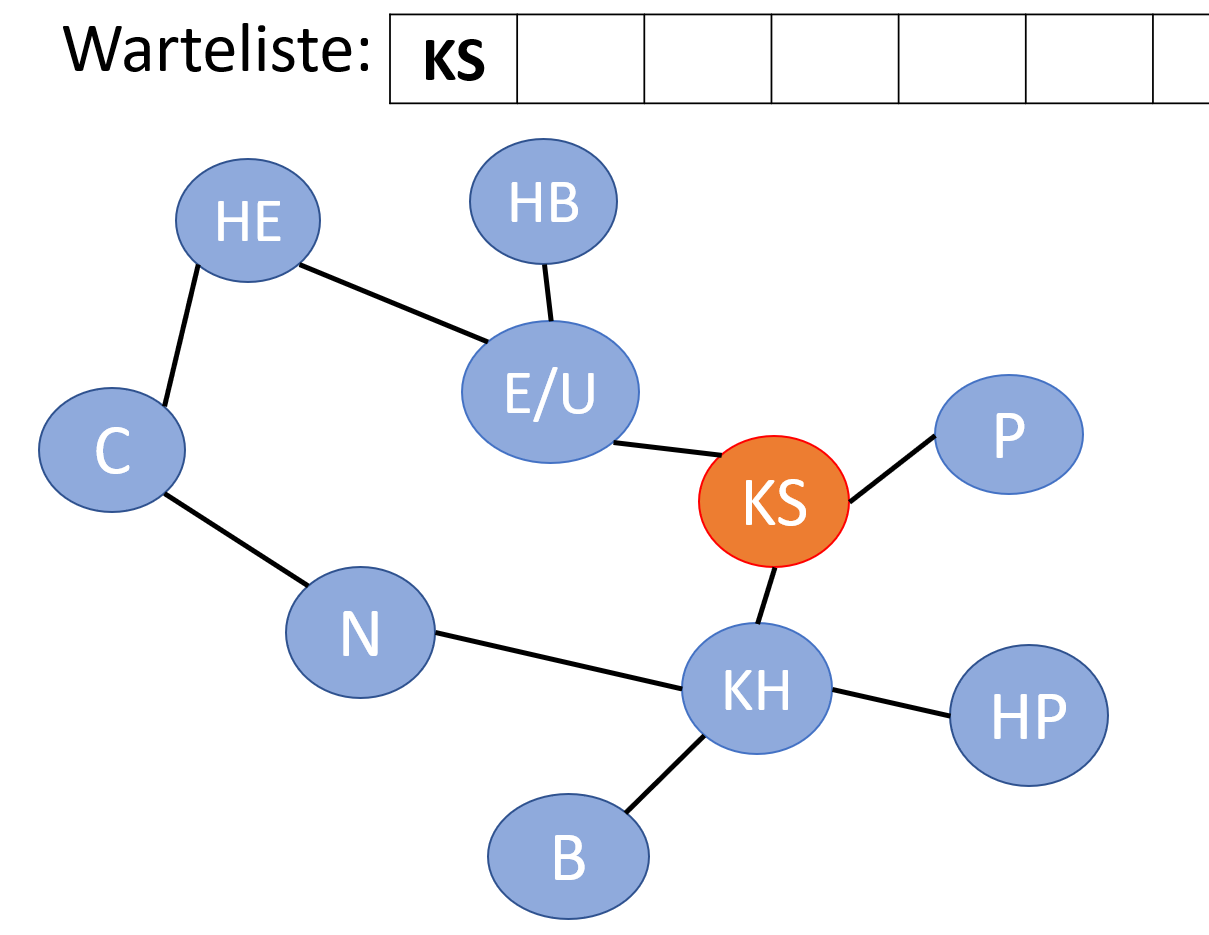
\includegraphics[width=\textwidth]{Pictures/BS/BFSB1.PNG}
    \caption{Die Breitensuche beginnt beim Startknoten {\bf{KS}}. Im ersten Schritt schreiben wir diesen auf unsere Warteliste und markieren ihn als besucht.}
    \label{fig:BS1}
    \end{subfigure}
    \vspace{5mm}
    \qquad
    \begin{subfigure}[h]{0.45\textwidth}
    \raggedleft
    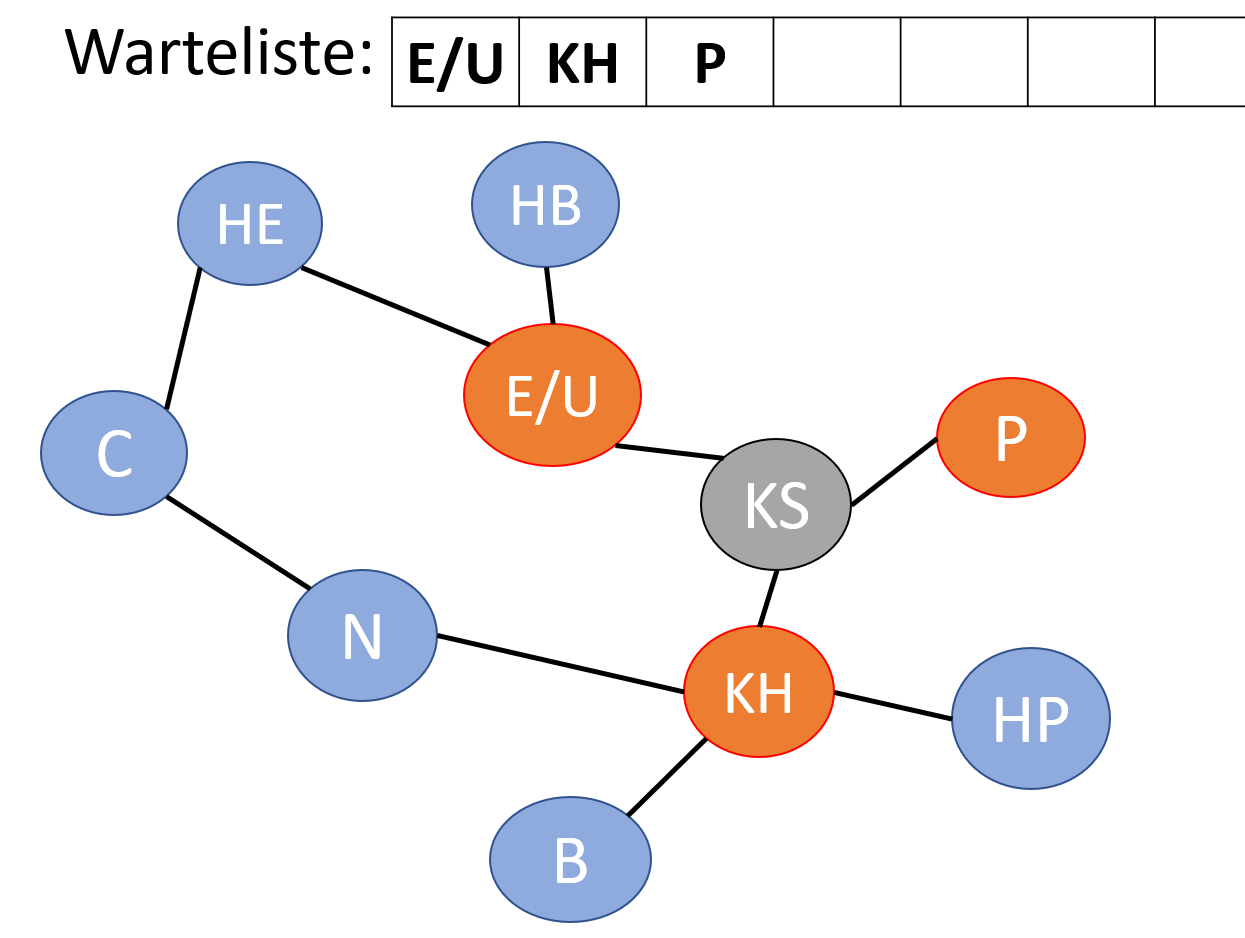
\includegraphics[width=\textwidth]{Pictures/BS/BFSB.PNG}
    \caption{Wir entfernen {\bf{KS}} aus der Warteliste und färben ihn darum grau. Als nächstes wollen wir die direkt benachbarten Haltestellen betrachten, wir schreiben sie also alphabetisch geordnet auf die Warteliste und markieren sie als besucht.}
    \label{fig:BS2}
    \end{subfigure}
    \vspace{5mm}
    \begin{subfigure}[h]{0.45\textwidth}
    \raggedright
    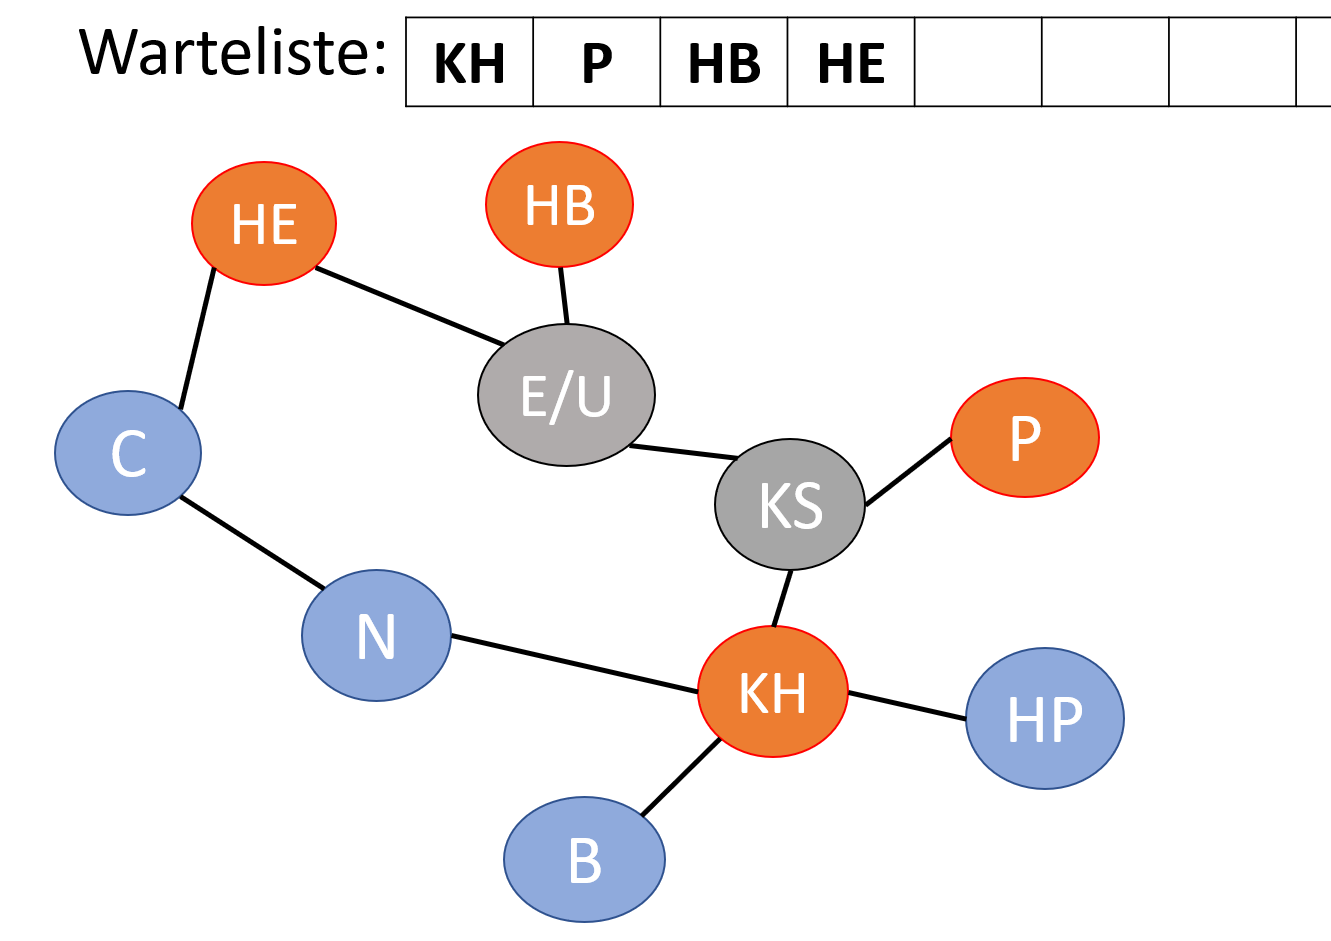
\includegraphics[width=\textwidth]{Pictures/BS/BFSB2.PNG}
    \caption{ Der erste Knoten auf der Warteliste war {\bf{E/U}} wir entfernen ihn und hängen seine zwei unbesuchten Nachbarn der Warteliste an.}
    \end{subfigure}
    \vspace{5mm}
    \qquad
    \begin{subfigure}[h]{0.45\textwidth}
    \raggedleft
    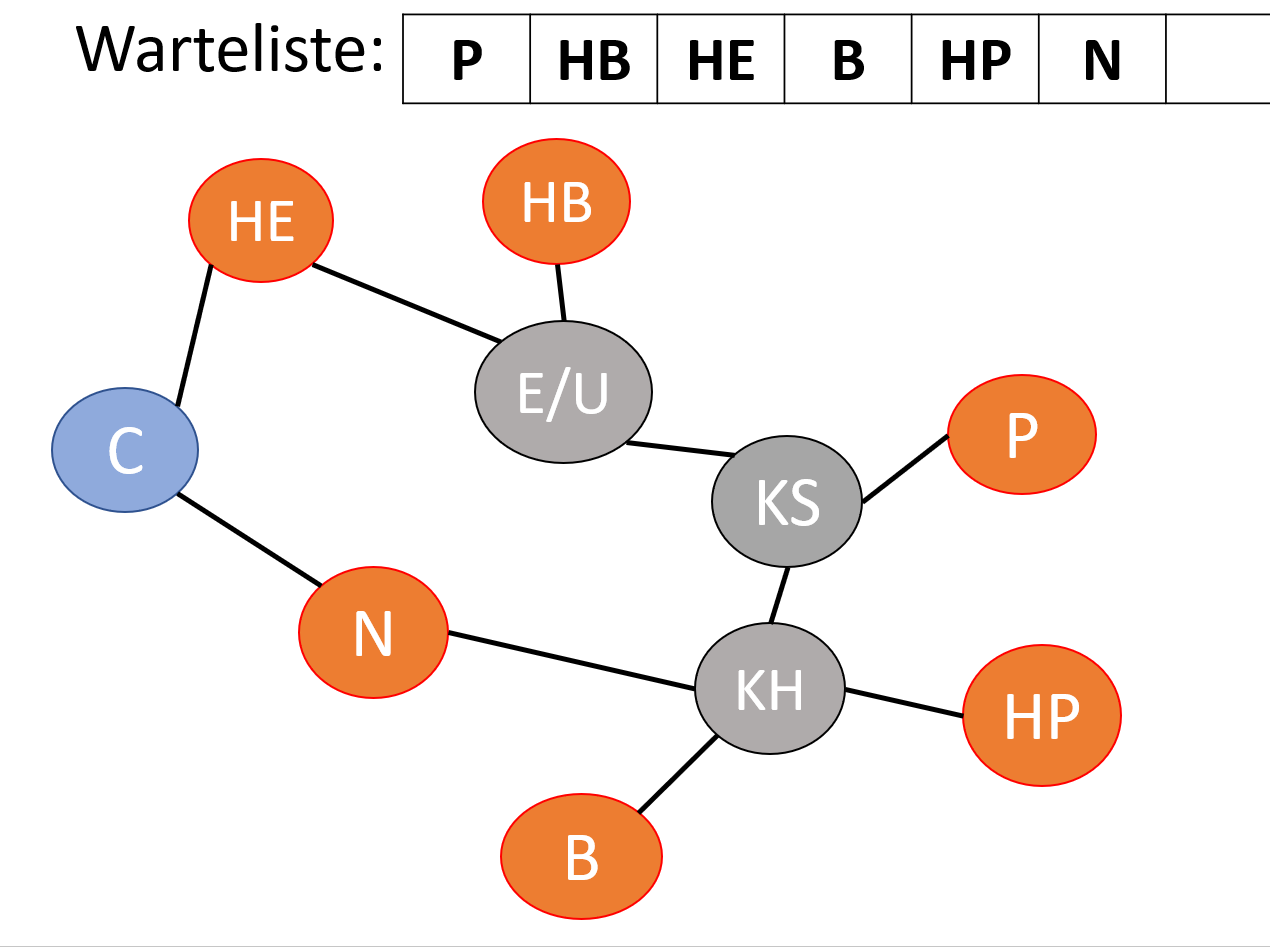
\includegraphics[width=\textwidth]{Pictures/BS/BFSB3.PNG}
    \caption{Der erste Knoten auf der Warteliste war {\bf{KH}}, wir entfernen ihn und hängen seine drei unbesuchten Nachbarn der Warteliste an.} 
    \end{subfigure}
    \end{figure}
\begin{figure}[H]\ContinuedFloat
    \begin{subfigure}[h!]{0.45\textwidth}
    \centering
    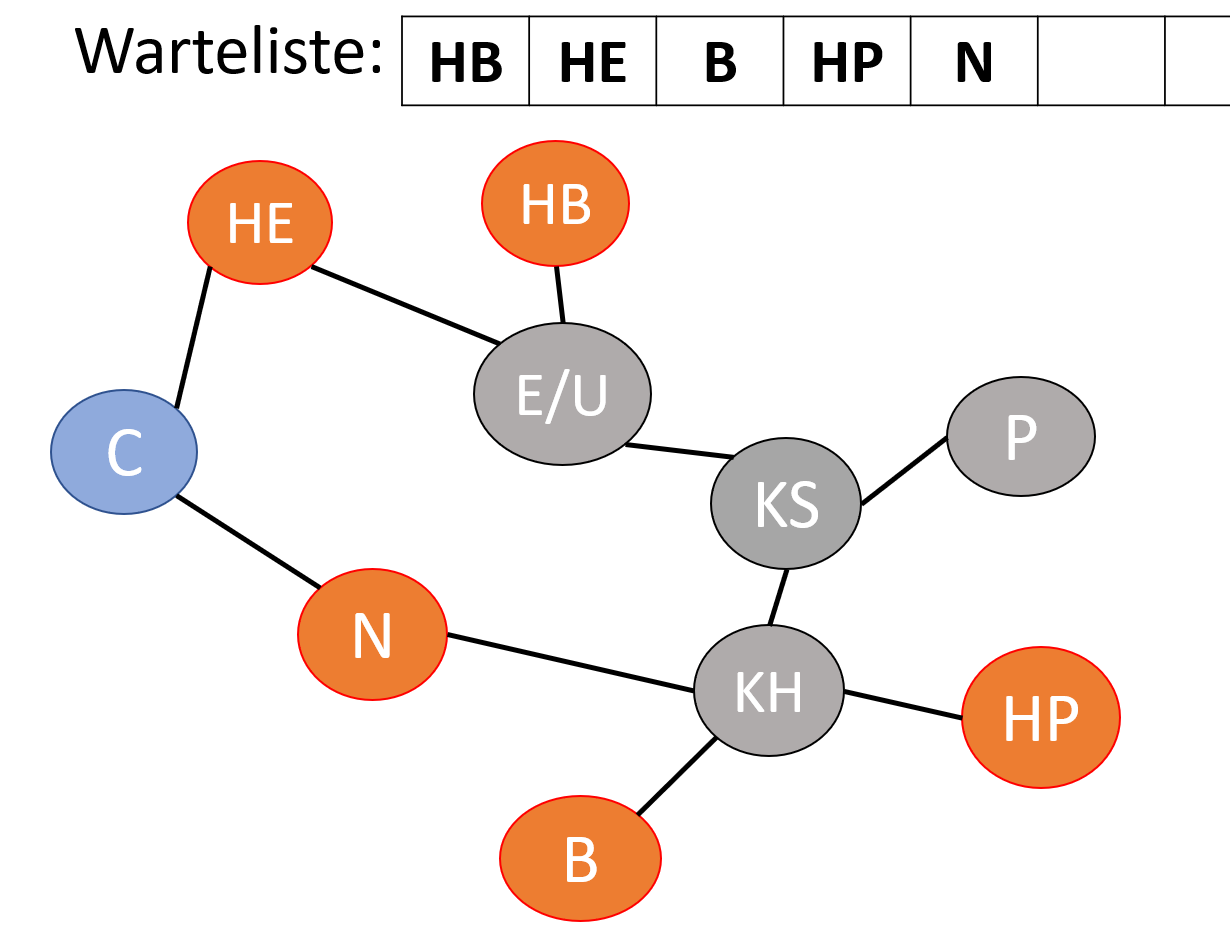
\includegraphics[width=\textwidth]{Pictures/BS/BFSB4.PNG}
    \caption{Als letzten Nachbarn von {\bf{KS}} können wir {\bf{P}} von der Warteliste entfernen. Er hat keine weiteren unbesuchten Nachbarn.} 
    \end{subfigure}
    \vspace{5mm}
    \qquad
    \begin{subfigure}[h]{0.45\textwidth}
    \centering
    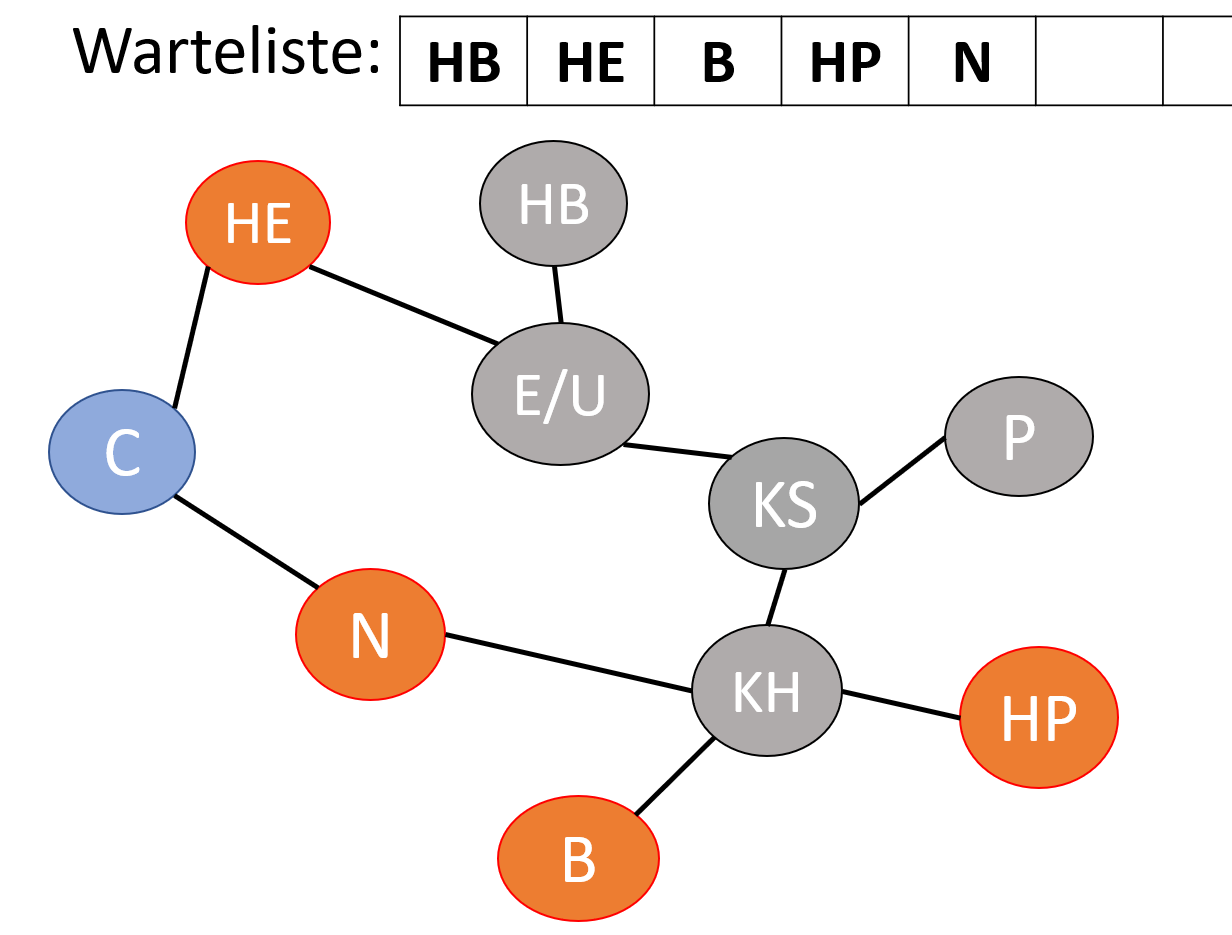
\includegraphics[width=\textwidth]{Pictures/BS/BFSB5.PNG}
    \caption{Als nächstes stehen in der Warteschlange die Nachbarn von {\bf{E/U}}. Wir entfernen zuerst {\bf{HB}} und müssen keine Knoten der Warteliste anhängen.}
    \end{subfigure}
    \vspace{5mm}
    \begin{subfigure}[h]{0.45\textwidth}
    \centering
    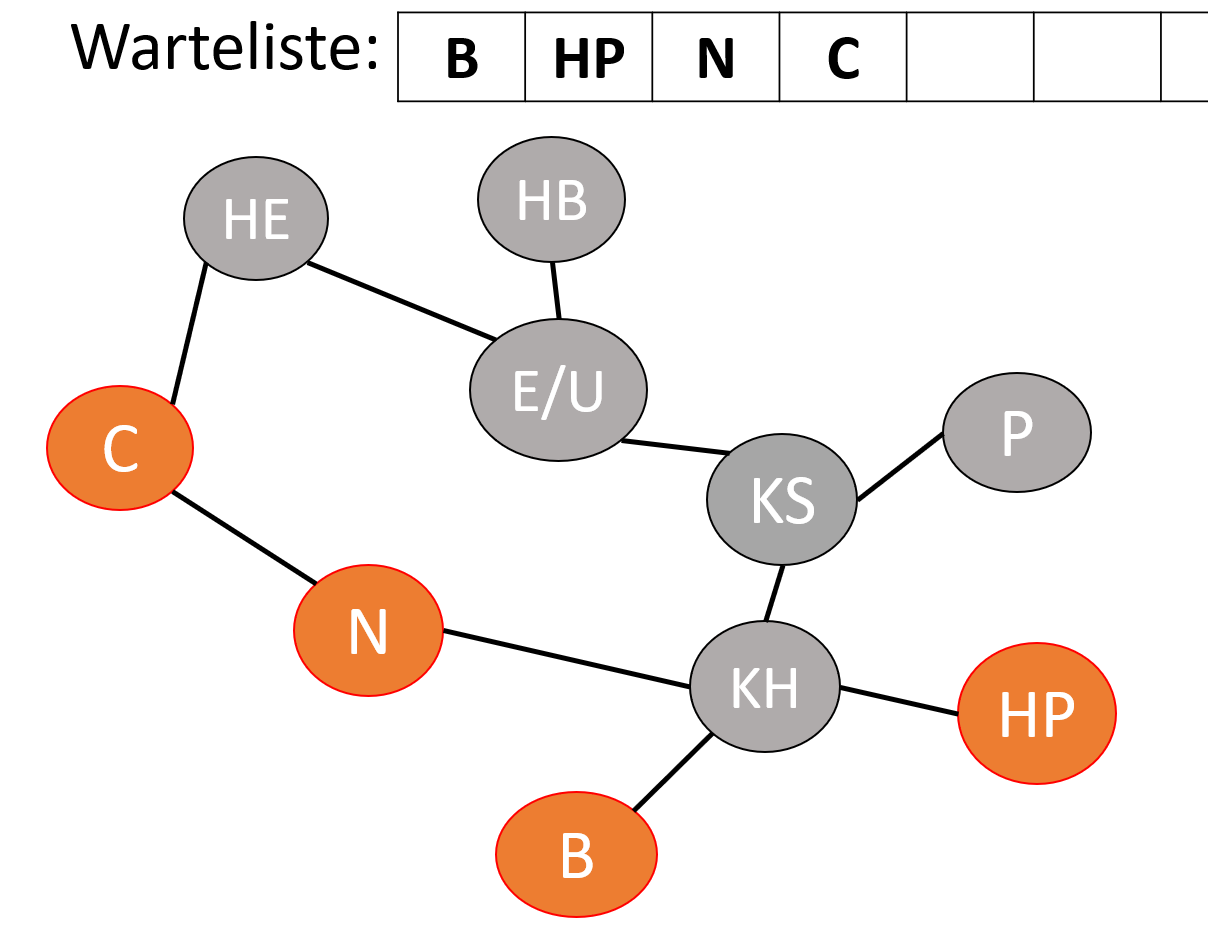
\includegraphics[width=\textwidth]{Pictures/BS/BFSB6.PNG}
    \caption{Wir entfernen {\bf{HE}} von der Warteliste, und hängen seinen unbesuchten Nachbarn {\bf{C}} der Warteliste an.}
    \end{subfigure}
    \qquad
    \begin{subfigure}[h]{0.45\textwidth}
    \centering
    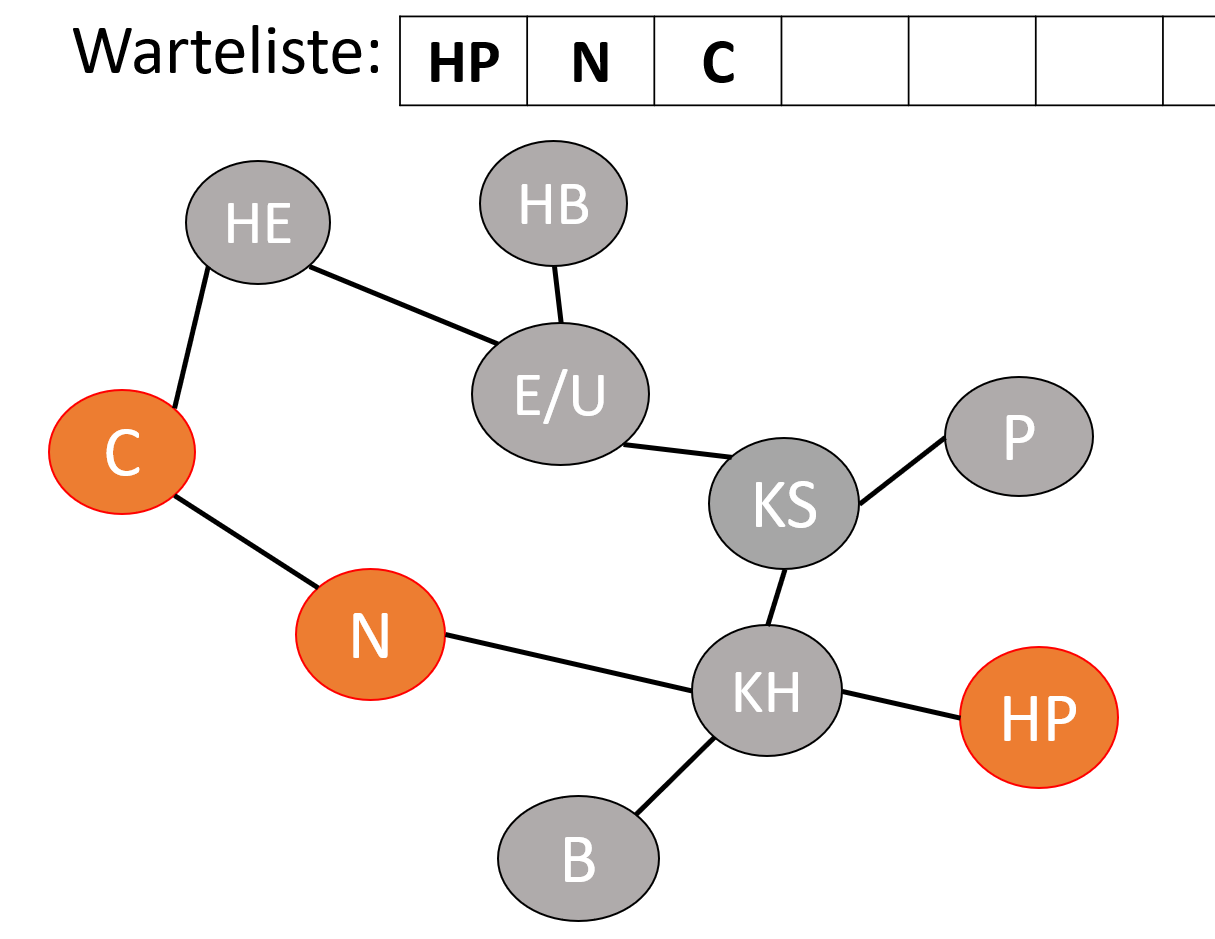
\includegraphics[width=\textwidth]{Pictures/BS/BFSB7.PNG}
    \caption{Wir entfernen {\bf{B}} aus der Warteliste. Der Knoten hat keine unbesuchten Nachbarn.}
    \end{subfigure}
\end{figure}
\begin{figure}[H]\ContinuedFloat
    \begin{subfigure}[h]{0.45\textwidth}
    \centering
    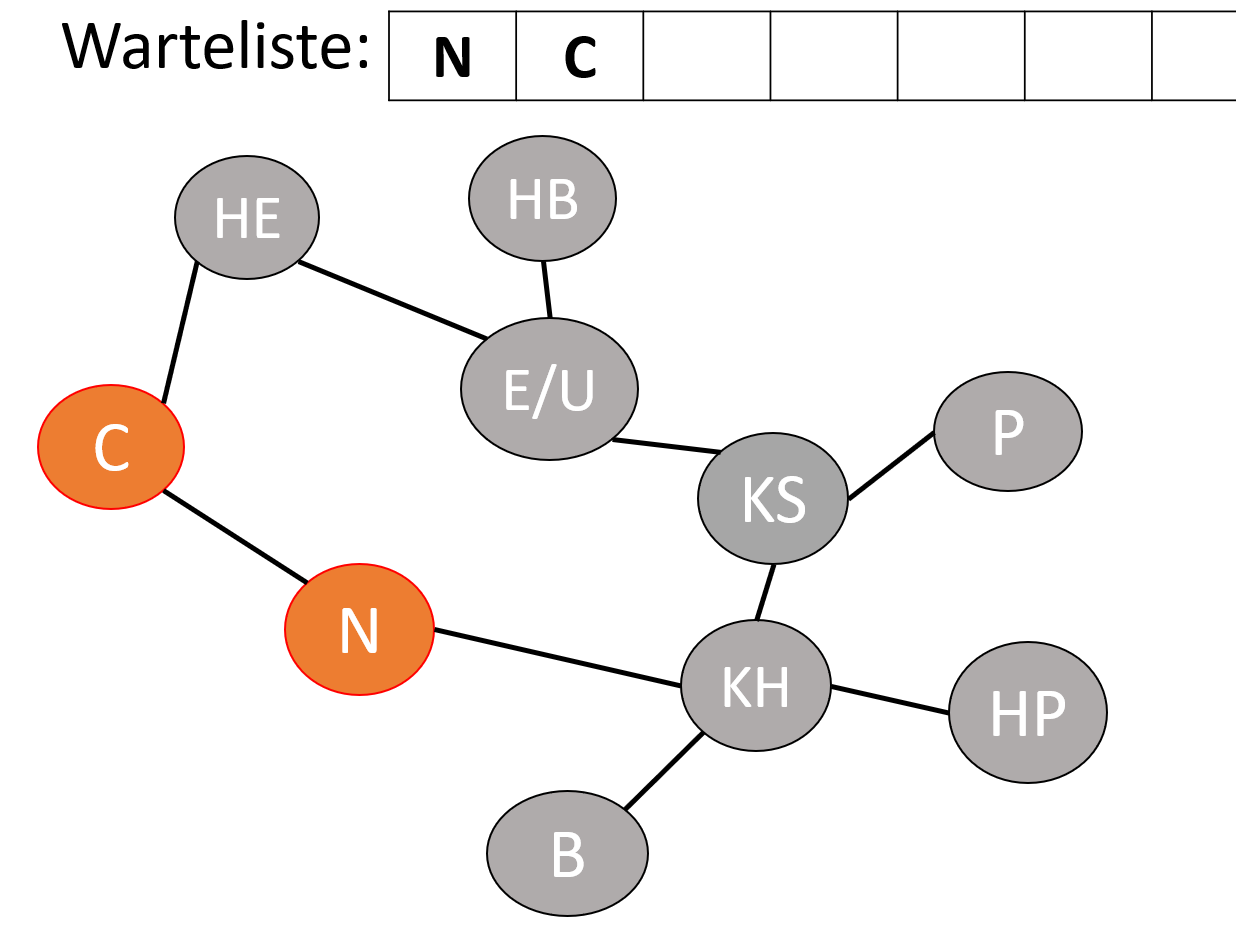
\includegraphics[width=\textwidth]{Pictures/BS/BFSB8.PNG}
    \caption{Wir entfernen {\bf{HP}} aus der Warteliste. Der Knoten hat keine unbesuchten Nachbarn.}
    \end{subfigure}
    \qquad
    \begin{subfigure}[h]{0.45\textwidth}
    \centering
    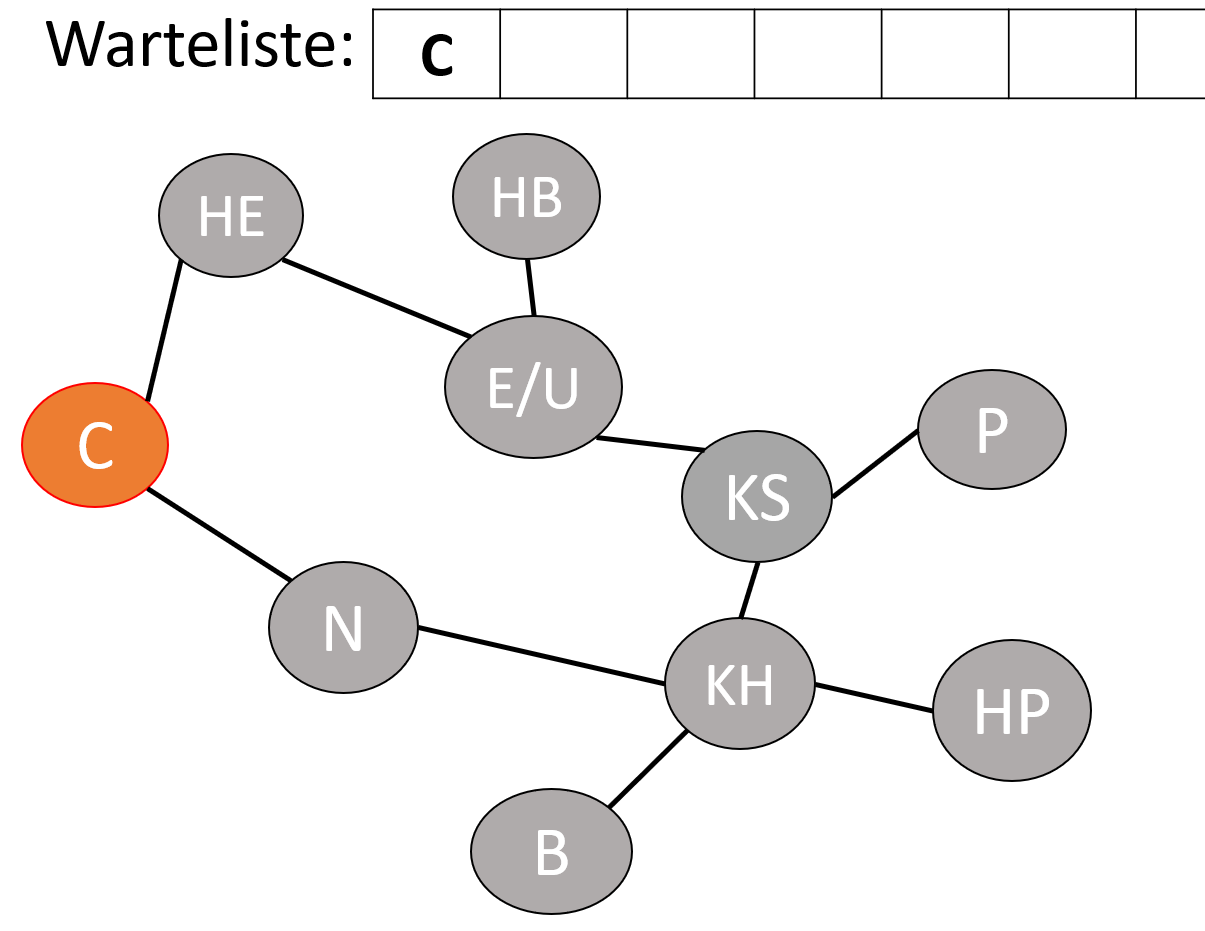
\includegraphics[width=\textwidth]{Pictures/BS/BFSB9.PNG}
    \caption{Als letzten Nachbarn von {\bf{KH}} können wir {\bf{N}} von der Warteliste entfernen. Die Nachbarn von {\bf{N}} sind alle bereits als besucht markiert. }
    \end{subfigure}
\end{figure}
\begin{figure}[H]\ContinuedFloat
     \centering
     \begin{subfigure}[h]{0.45\textwidth}
    \centering
    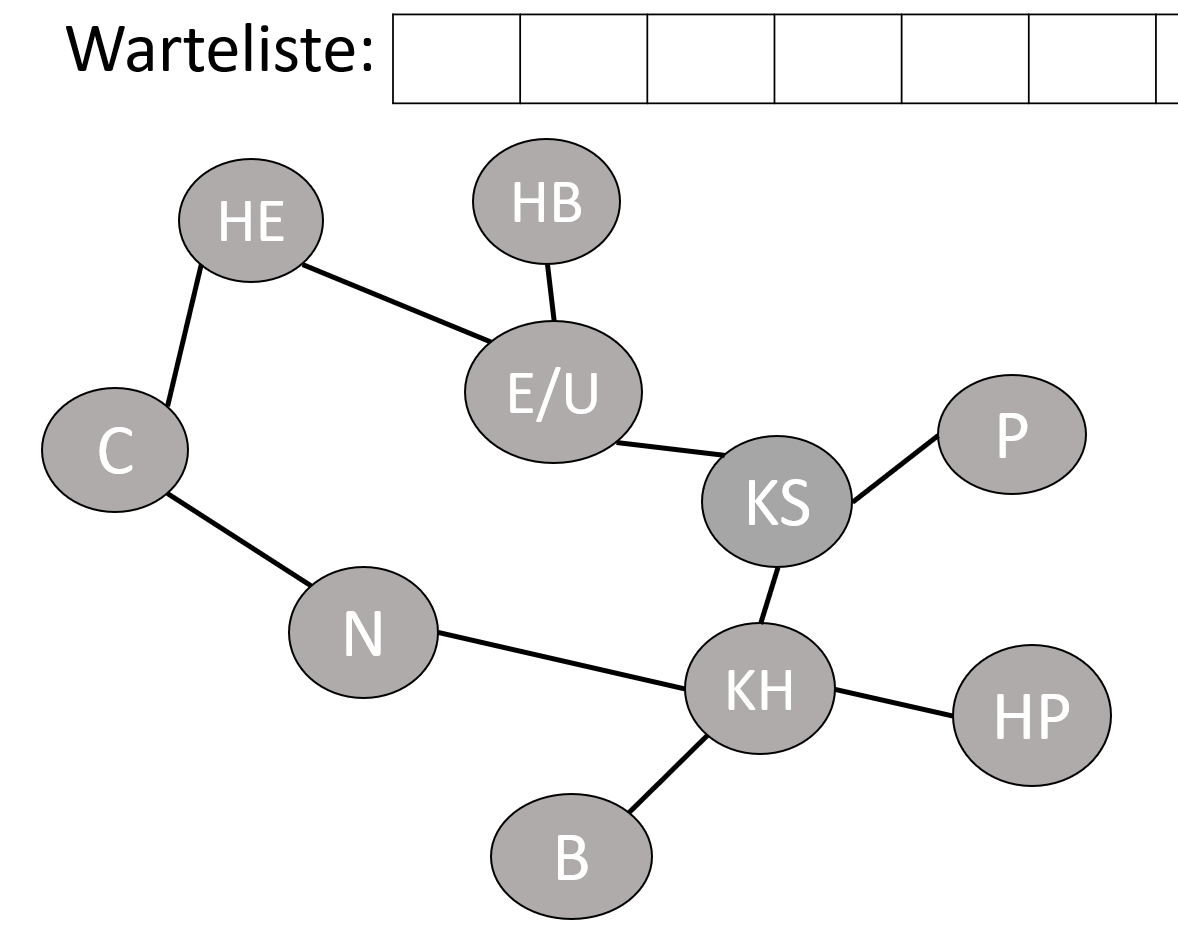
\includegraphics[width=\textwidth]{Pictures/BS/BFSB10.PNG}
    \caption{Zuletzt entfernen wir {\bf{C}} aus der Warteliste. Seine Nachbarn wurden alle bereits einmal besucht und die Warteliste ist jetzt leer. Der Algorithmus endet also an dieser Stelle.}
    \end{subfigure}
\end{figure}
Die Breitensuche besucht die Knoten also in der Reihenfolge 
$$ \text{ \bf{KS,E/U,KH,P,HB,HE,B,HP,N,C}} $$

\subsection{Der Algorithmus in Worten}
Wir wollen nun den Suchalgorithmus, welchen wir oben graphisch an einem Beispiel aufgezeichnet haben, allgemein formalisieren. In einer ersten Version geben wir dem Algorithmus keine Abbruchsbedingung, das heisst die Breitensuche läuf weiter, bis alle möglichen Knoten einmal besucht wurden. Um uns jeweils zu merken, welche Knoten wir als nächstes betrachten wollen, verwenden wir eine Warteliste. Um uns zu merken, welche Knoten wir bereits betrachtet haben, markieren wir diese als besucht. So können wir vermeiden, dass ein Knoten mehrmals bearbeitet wird.\\

 \noindent {\bf{Input:}} Ein Graph $G=(V,E)$ und ein Startknoten $s \in V$.

\noindent {\bf{Output:}} Die Knoten von $G$ aufsteigend geordnet nach Abstand zum Startknoten $s$.

\begin{enumerate}
    \item Schreibe den Startknoten $s$ auf die Warteliste und markiere ihn als besucht.
    \item Entferne den ersten Knoten von der Warteliste und prüfe für jeden Nachbarn, ob er bereits als besucht markiert wurde.
    \item Falls nicht, hänge ihn der Warteliste an und markiere ihn als besucht.
    \item Wiederhole die Schritte 2 und 3 bis keine Knoten mehr auf der Warteliste sind.
\end{enumerate}

\begin{aufgabe} \label{newinitial}
In welcher Reihenfolge besucht die Breitensuche die Haltestellen, wenn wir statt bei der Kantonsschule beim Bellvue starten?
\end{aufgabe}

\begin{aufgabe} \label{directed}
Wir betrachten immer noch den Graphen in Abbildung \ref{fig:BS1}. Nun
treten bei verschiedenen Trams technische Störungen auf, so dass die Strecken Bellvue - Platte und Central - Hottingerplatz jeweils nur noch in dieser einen Richtung befahren werden können. Zeichne den gerichteten Graphen (mit den gleichen 10 Knoten) der zu dieser Situation passt. In welcher Reihenfolge besucht die Breitensuche jetzt die Knoten wenn wir wieder beim Bellvue starten? 
\end{aufgabe}


Alice und Bob spielen das Wikipedia-Spiel. Es funktioniert wie folgt: Alice gibt Bob zwei Wikipedia-Artikel vor und dieser muss durch das Klicken von möglichst wenigen Links von einem Artikel zum anderen kommen. Wir können Wikipedia als Graphen darstellen, indem wir für jeden Artikel einen Knoten zeichnen und für einen Link in Artikel $A$ zu Artikel $B$ eine gerichtete Kante von $A$ nach $B$. Der tatsächliche Graph von allen deutschen Wikipedia-Artikeln hat so fast 2.5 Millionen Knoten und noch viel mehr Kanten. Wir betrachten nur einen sehr kleinen Ausschnitt davon mit den folgenden Artikeln:
\begin{multicols}{2}
\begin{itemize}
    \item {\bf{B}}: Bellvue
    \item {\bf{BS}}: Breitensuche
    \item {\bf{D}}: Deutschland
    \item {\bf{E}}: Eisenbahn
    \item {\bf{G}}: Graph
    \item {\bf{K}}: Knoten
    \item {\bf{L}}: Laufzeit
    \item {\bf{S}}: Schweiz
    \item {\bf{SBZ}}: Strassenbahn Zürich
    \item {\bf{U-B}}: U-Bahn
    \item {\bf{Z}}: Zürich
\end{itemize}

\end{multicols}
mit dem zugehörigen gerichteten Graphen:
\begin{figure}[h!]
    \centering
    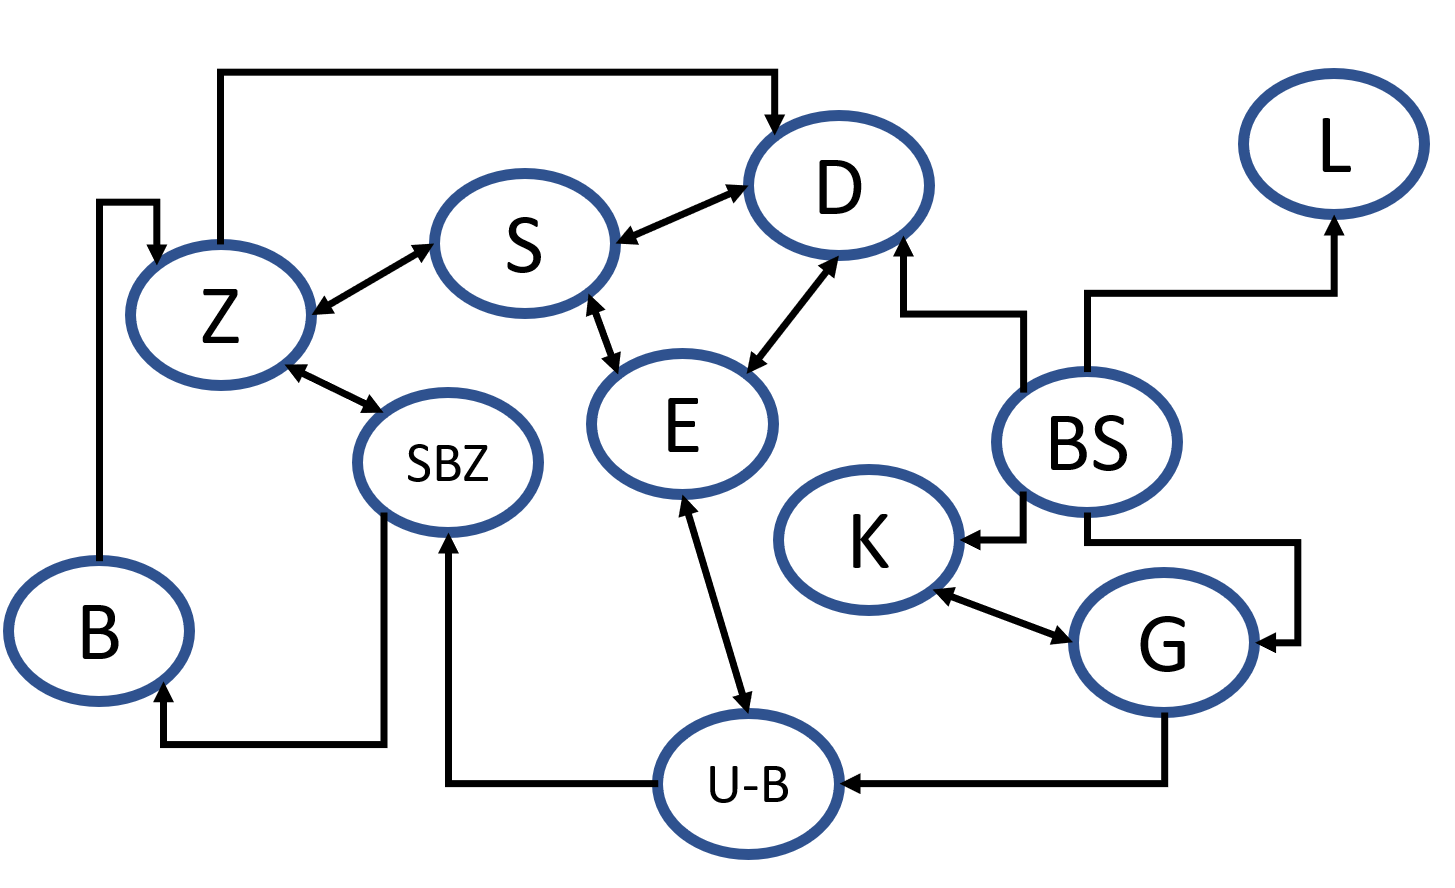
\includegraphics[scale=0.5]{Pictures/Wikipedia.PNG} 
    \caption{Die Verlinkung von Wikipedia-Artikeln als Graph.}
    \label{fig:my_label}
\end{figure}

\begin{aufgabe} \label{Wikipedia}
Alice sagt zu Bob: ''Öffne den Wikipedia-Artikel über die Breitensuche und finde den Artikel über die Strassenbahnen von Zürich.'' Wenn Bob nur die 11 aufgelisteten Artikel zur Verfügung hat, kann er dann den gewünschten Artikel erreichen? Verwende die Breitensuche um die Frage zu beantworten.
\end{aufgabe}

In Aufgabe \ref{Wikipedia} haben wir eine Abbruchsbedingung in Form eines gesuchten Knotens. Wir können also der Breitensuche als Input zusätzlich zum Graphen und Startknoten noch einen Zielknoten geben und den Algorithmus abbrechen, sobald der Zielknoten als besucht markiert wurde.

Jetzt wäre es natürlich schön wenn wir den Algorithmus so abändern könnten, dass er uns zusätzlich sagt, wieviele Klicks Bob mindestens braucht und was eine mögliche optimale Lösung wäre. Doch bevor wir dieses Problem lösen, wollen wir zuerst die Breitensuche in Python implementieren.

\subsection{Der Algorithmus in Python}
Wir wollen ein Programm für die Breitensuche schrieben und dieses gleich an unserem Tramlinienbeispiel testen.
Da wir uns bei der Breitensuche jeweils für jeden Knoten alle seine Nachbarn merken (bzw. auf die Warteliste schreiben) müssen, bietet es sich an die ''Liste der Nachbarn''- Darstellung für die Graphen zu verwenden.
In Python implementieren wir einen Graphen also am besten als eine Menge von Listen. Der Graph in Abbildung \ref{fig:BS1} wäre zum Beispiel:

\begin{figure}[H]
    \centering
    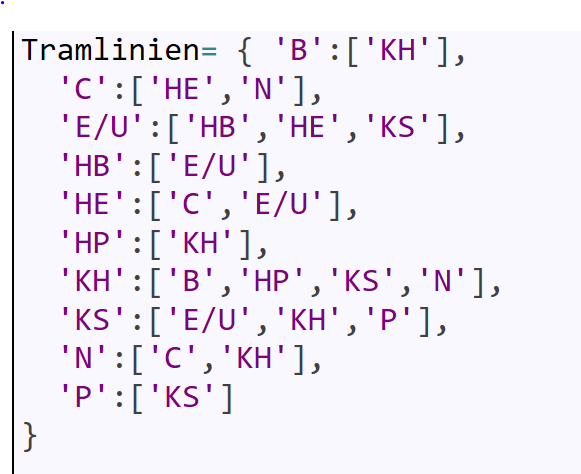
\includegraphics[scale=0.8]{Pictures/ListeDerNachbarn.PNG}
    \caption{Tramliniengraph in der ''Liste der Nachbarn''-Darstellung}
    \label{fig:Tram2}
\end{figure}

Tippe das Programm in Abbildung \ref{fig:Breitensuche} ab. Vergleiche die Ausgabe mit der Reihenfolge der Knoten die wir im Abschnitt 2.1 gefunden haben.

\begin{figure}[H]
    \centering
    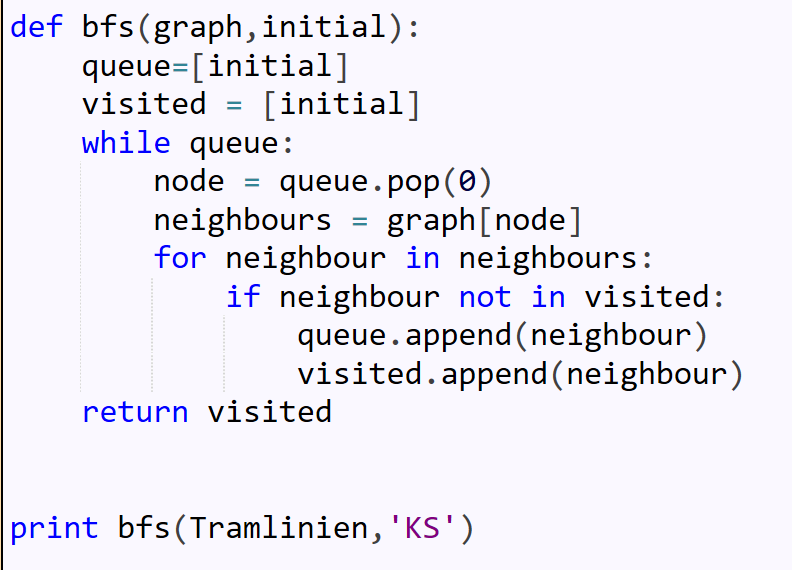
\includegraphics[scale=0.8]{Pictures/Breitensucheprog.PNG}
    \caption{Breitensuche in Python}
    \label{fig:Breitensuche}
\end{figure}

Wir nennen das Programm ''bfs'' für ''breadth first search'' (englischer Name der Breitensuche). 

\begin{aufgabe} \label{ProgFragen} Beantworte folgende Fragen zum Programm in Abbildung \ref{fig:Breitensuche}
\begin{itemize} 
    \item Wofür brauchen wir die Listen ''queue'' und ''visited''?
    \item Welche Zeilen im Programm entsprechen welchem Schritt des Algortihmus in Abschnitt 2.1?
\end{itemize}
\end{aufgabe}

\paragraph{Die Laufzeit} hängt bei einem Algorithmus für Graphen davon ab, wieviele Knoten und Kanten dieser hat. Falls die Breitensuche durch den ganzen Graphen $G=(V,E)$ läuft, so durchlaufen wir die while-Schlaufe für jeden Knoten einmal, also insgesammt $|V|$-mal. In der for-Schlaufe betrachten wir jeweils jede ausgehende Kante, insegsamt durchlaufen wir sie also maximal (bei einem ungerichteten Graphen) $2|E|$-mal. Die Laufzeit der einzelnen Schritte ist immer $\mathcal{O}(1)$. Wir erhalten eine Gesamtlaufzeit von $\mathcal{O}(|V|+|E|)$. Die Zeit, welche der Computer benötigt um die Breitensuche durchzuführen, wächst also linear in der Anzahl der Knoten und Kanten des Graphens an.

\paragraph{Der Speicherplatzverbrauch} der Breitensuche ist $\mathcal{O}(|V|)$ da wir alle bisher besuchten Knoten speichern. Sobald du mehrere Algorithmen für Graphen kennst kannst du sie anhand ihrer Laufzeiten und ihrem Speicherplatzverbrauch miteinander vergleichen.

\begin{aufgabe}  \label{WikiProgAufg} {\bf{*}}
Ändere das Programm ''bfs'', so dass es abbricht sobald ein gesuchter Knoten gefunden wurde und überprüfe damit deine Lösung von Aufgabe \ref{Wikipedia}. Nenne das neue Programm ''bfs\_goal''.
\end{aufgabe}

\paragraph{Lernaufgabe}
Alice und Bob haben eine Datenbank ('Familien') zur Verfügung in welcher für jeden Menschen jeweils die Eltern und die Kinder aufgeführt sind. Sie geht 6 Generationen zurück. Nun fragen sie sich ob sie eine gemeinsame Ur-ur-ur-ur-Grossmutter haben. 
\begin{enumerate}
    \item Wie können sie die Daten als ungerichteten Graphen darstellen?
    \item Wie können sie die Antwort zu ihrer Frage mit Hilfe des Programms ''bfs\_goal'' finden? Beschreibe deine Idee in Worten. (noch nicht programmieren)
\end{enumerate}
Nun wollen sie ein Programm welches ihnen statt der Liste aller besuchten Knoten als Ausgabe einfach mitteilt ob sie eine gemeinsame Ur-ur-ur-ur-Grossmutter haben und zwar in Form einer Ausage wie: '' Der Startknoten und der Endknoten sind in \dots '' oder ''Der Startknoten und der Endknoten sind nicht in \dots''
\begin{enumerate}[resume]
    \item Was kommt in die Lücke des gewünschten Outputs?
    \item Schreibe das Programm und teste es an einem kleinen Graphen.
\end{enumerate}

\subsection{Kontrollfragen}
\begin{enumerate}
    \item Wie würdest du einem Mitschüler, welcher diesen ersten Teil der Stunde verpasst hat in wenigen Sätzen erklären, was die Breitensuche ist?
    \item Du kennst bereits viele verschiedene Zusammenhänge, welche sich als Graphen darstellen lassen. Überlege dir eine ''Alltagssituation'', bei der du die Breitensuche verwenden könntest.
\end{enumerate}
Welche der folgenden Schüler haben recht? Welche nicht? Begründe!
\begin{enumerate}[resume]
    \item David sagt:''Es gibt bestimmt Graphen bei denen ein Knoten im Laufe der Breitensuche mehr als einmal in der Warteliste auftaucht.''
    \item Fred behauptet: ''Ob ich einen bestimmten Knoten in einem zusammenhängeden Graphen finden kann hängt nicht davon ab welchen Startknoten ich gewählt habe.''
    \item * Gregory meint: '' Ich kann einen zusammenhängenden Graphen mit beliebig vielen Knoten zeichnen und den Startknoten so wählen, dass nie mehr als ein Knoten auf der Warteliste steht.
\end{enumerate}

\newpage